\section{Installazione}
\label{sec:installazione}

Per installare l'applicazione è necessario scaricare il codice sorgente dal \glossario{repository} in una cartella dedicata.\\
Il \glossario{repository} è disponibile a questo link - \href{https://github.com/ALT-F4-eng/ArtificialQI}{https://github.com/ALT-F4-eng/ArtificialQI}
Per scaricare il codice sorgente vi sono due modalità principali:
\begin{itemize}
    \item Scaricare il repository in formato zip e decomprimerlo in una cartella dedicata
    \item Clonare il repository tramite il seguente comando:\\
     git clone https://github.com/ALT-F4-eng/ArtificialQI.git
\end{itemize}

\section{Avvio}
\label{sec:avvio}

L’applicazione può essere avviata, dopo essersi posizionati con il terminale nella cartella del progetto, tramite i seguenti comandi:
\begin{itemize}
    \item docker compose build
    \item docker-compose up
\end{itemize}
Una volta avviata l’applicazione, è possibile accedervi tramite il browser all’indirizzo http://localhost:4200.

\section{Utilizzo}
\label{sec:utilizzo}

La sezione seguente presenta le funzionalità del sistema.

\subsection{Sezione Home}
\label{subsec:sezione_home}

La sezione Home è una pagina interamente descrittiva che presenta le funzionalità generali dell'applicazione.

\subsection{Sezione Dataset}
\label{subsec:sezione_dataset}

\begin{figure}[H]
    \centering
    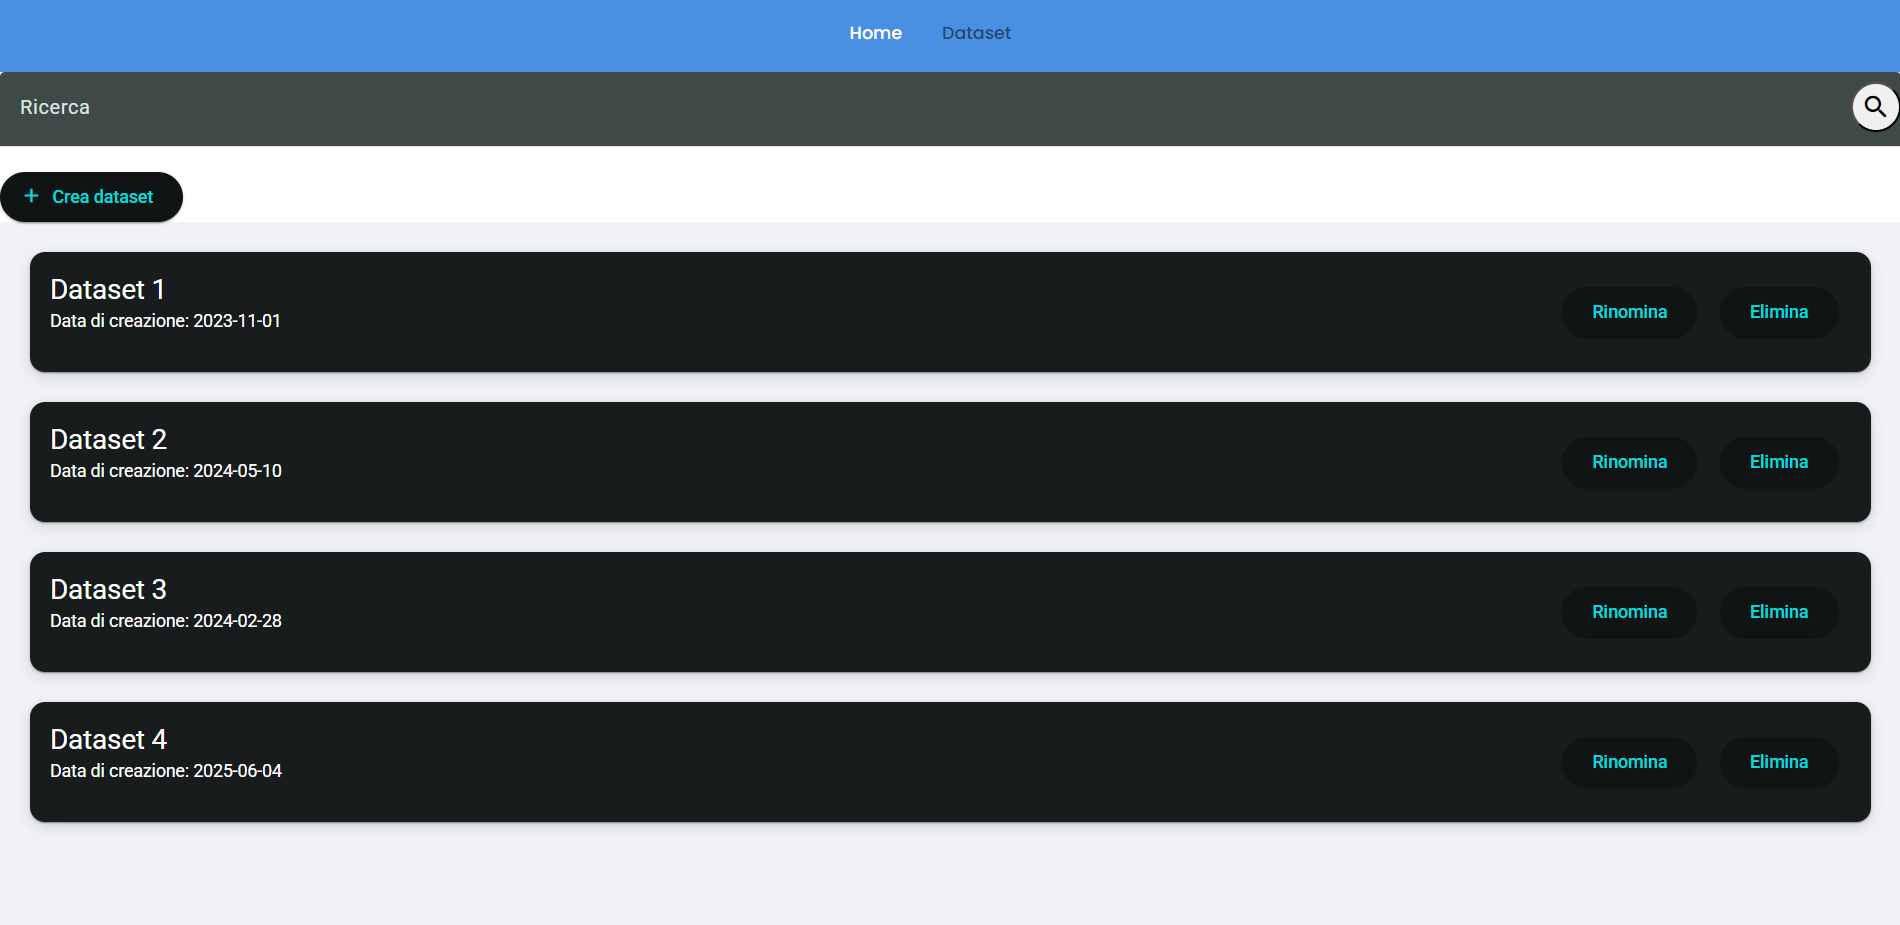
\includegraphics[scale=0.35]{Sezioni/Requisiti/immagini/dataset.png}
\end{figure}

La sezione Dataset è composta da tre elementi principali:
\begin{itemize}
    \item Barra di ricerca - Attraverso la barra di ricerca posizionata nella parte superiore della pagina è possibile filtrare la lista dei dataset per nome.
    \item Bottone crea dataset - Attraverso il bottone crea dataset è possibile aggiungere un nuovo dataset alla lista attraverso un form pop-up che richiederà l'inserimento di un nome.
    \begin{figure}[H]
    \centering
    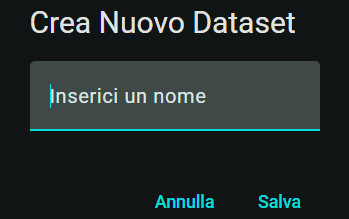
\includegraphics[scale=0.6]{Sezioni/Requisiti/immagini/nuovo_dataset.png}
    \end{figure}
    \item Lista dataset - Qui saranno visualizzati tutti i dataset salvati con i relativi bottoni che consentono di rinominare un dataset oppure eliminarlo con una richiesta pop-up.
    \begin{figure}[H]
    \centering
    
    \begin{minipage}[b]{0.48\textwidth}
        \centering
        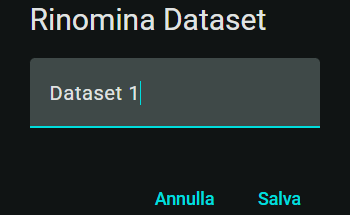
\includegraphics[scale=0.5]{Sezioni/Requisiti/immagini/rinomina_dataset.png}
    \end{minipage}
    \hfill
    \begin{minipage}[b]{0.48\textwidth}
        \centering
        
\includegraphics[scale=0.5]{Sezioni/Requisiti/immagini/elimina_dataset.png}
    \end{minipage}
    \end{figure}
\end{itemize}
Infine il sistema notificherà l'utente con l'esito di ogni operazione fornendo una conferma o un errore in modo dinamico.
\begin{figure}[H]
    \centering
    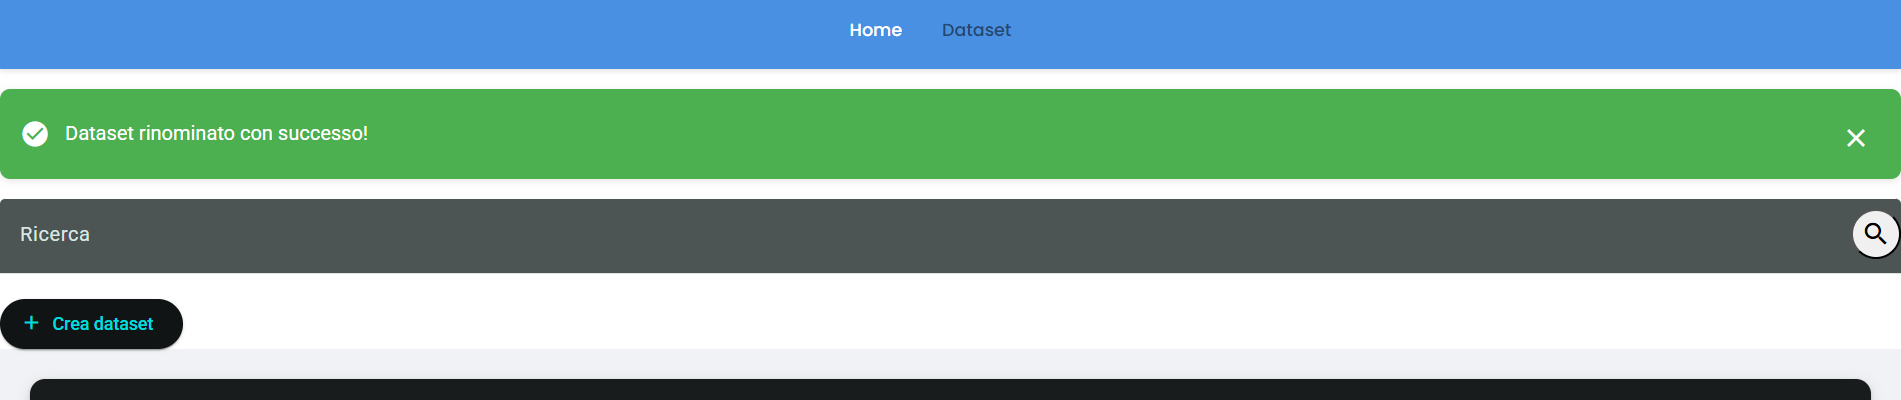
\includegraphics[scale=0.35]{Sezioni/Requisiti/immagini/notificav.png}
\end{figure}
\begin{figure}[H]
    \centering
    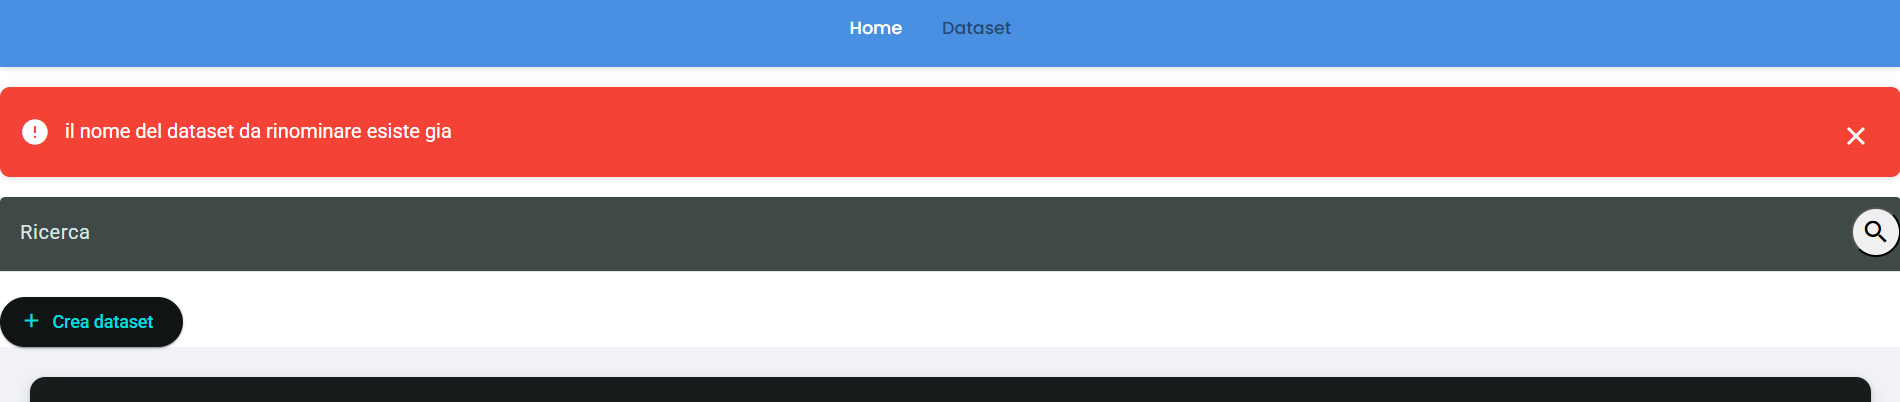
\includegraphics[scale=0.35]{Sezioni/Requisiti/immagini/notificax.png}
\end{figure}